\documentclass[12pt, a4paper]{article}
\usepackage{amsmath}
\usepackage{amsfonts}
\usepackage{amsthm}
\usepackage{mathtools}
\newtheorem{theorem}{Theorem}[section]
\newtheorem{definition}{Definition}[section]
\numberwithin{equation}{section}
\usepackage{pgfplots}
\pgfplotsset{width=10cm,compat=1.9}
\graphicspath{ {img/} }
\DeclareGraphicsExtensions{.png,.jpg}

\title{Perceptrons}
\author{Kristian Wichmann}

\begin{document}
\maketitle

\section{Definition}
A \textit{perceptron} is the simplest possible linear feed-forward neural net. It is a binary classifier consisting of a list of input features feeding into one, linear threshold binary neuron.

So, if there's $n$ features, a data point $x$ is a $n$-dimensional vector. The classifier is characterized by another $n$-dimensional weight vector $w$ and a constant $b$. The classification can be summed up as:
\begin{equation}
f(x)=\textrm{sign}(w^T x+b)
\end{equation}
Here, the two possible outcomes are +1 (positive) and -1 negative.

\subsection{Bias as a weight}
It is possible to treat $b$ as a weight term by making each sample vector into a $n+1$-dimensional one where the zero'th feature is simply a 1. Then $b$ is then simply the zero'th element of the weight vector. The classification algorithm can then be written:
\begin{equation}
f(x)=\textrm{sign}(w^T x)
\end{equation}

\section{Picking features vs. learning}
So if we wanted to set up a perceptron classifier, the first step would be to decide on the features. This is a step that is done by us - human beings - and thus no machine learning is happening in this step. But based on common sense and domain knowledge, a set of features is extracted from the raw input.

When that has been done, the training set is used for letting the perceptron learn appropriate values for $w$. This is the learning part of the perceptron.

\section{Training algorithm (for a separable training set)}
It turns out that if the training set is indeed linearly separable, then the following algorithm will always produce an appropriate weight vector $w$:
\begin{itemize}
\item Initialize the weight vector $w$
\item Start with $i=1$.
\item Inspect $x_i$ from the training set and do the following:
\begin{itemize}
\item Is $x_i$ correctly classified according to the current weights?
\item If yes, do nothing.
\item If $x_i$ is misidentified as a negative, then add $x_i$ to $w$.
\item If $x_i$ is misidentified as a positive, then subtract $x_i$ from $w$.
\end{itemize}
\item Increase $i$ by one. If you're at the end of the training set, set $i=1$. Repeat.
\end{itemize}
If indeed the training set is linearly separate (and this may not be the case!), then the weight vector $w$ will eventually correspond to one such classifier.

\subsection{Geometrical picture}
As a warm-up to the proof that the algorithm described above actually works, let's consider the situation geometrically.

We may view a given choice of weights $w$ as a vector in $n+1$ dimensional euclidean space. The decision boundary is then the hyperplane consisting of vectors perpendicular to $w$. Samples in the corresponding positive half-space 
are classified as positive, and samples in the corresponding negative half-space are classified as negative.

Conversely, we may consider a specific sample $x$. Then there will be some weight vectors which give the right prediction for $x$ and some which give the wrong prediction. Here, the hyperplane perpendicular to $x$ separates these two cases. If $x$ is actually positive, then $w$ lying in the positive half-space makes valid predictions. If $x$ is actually negative, $w$ lying in the negative half-space makes valid predictions. We're looking for a $w$ which lies on the "right side" of every hyperplane corresponding to points in the training set. Combining these conditions, we trace out a hyper-pyramid (of infinite height) in $n+1$-dimensional space\footnote{In general, there's no guarantee that such a hyper-pyramid exists, but we're working under the assumption that it does}.

\begin{figure}
\centering

\includegraphics{hyper_pyramid}
\caption{Example of the subset of feasible weights. Two training set samples are given. The blue region shows the half-space of weights which makes correct predictions for the first sample, and the red region similarly for the second sample. The region feasible for both is the purple region. In general, the solution set is a \textit{hyper-pyramid}, since all such planes go through the origin.}
\label{fig:hyper_pyramid}
\end{figure}

\subsubsection{Convexity}
Since the average of two vectors lying in this hyper-pyramid of solutions will itself lie in this region, the problem is said to be \textit{convex}. The hyper-pyramid is itself a convex shape.

\subsection{Loose proof}
The idea of the proof is this: We would like to show, that with each iteration which changes the weight vector, the euclidean distance to \textbf{every} feasible weight vector choice gets smaller. However, it turns out that this is not true.

\begin{figure}
\centering
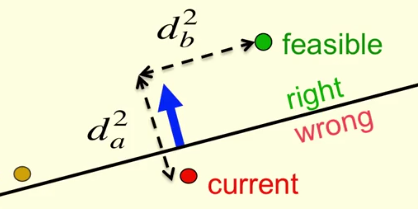
\includegraphics{perceptron_training}
\caption{A step in the perceptron training process.}
\label{fig:perceptron_training}
\end{figure}

To see why, take a look at figure \ref{fig:perceptron_training}. Here, the current weight are shown in red and the relevant training set sample is the blue arrow. Since this sample is currently misclassified, it will be added to the weights in this step of the training process. Clearly, this takes the weights closer to the green feasible weights. But the golden feasible weight is so close to the boundary, that the distance to it does not actually decrease!

So it seems we cannot make sure that the distance to \textbf{all} feasible weigh points gets smaller in the training step. Let's ease the condition to \textit{generously feasibly} weight vectors. Figure \ref{fig:generously_feasible} shows such a generously feasible region: We've introduced a margin with a width equal to the length of the training sample vector. Surely now, the new weight vector will be closer to all the generously feasible weight vectors.

\begin{figure}
\centering
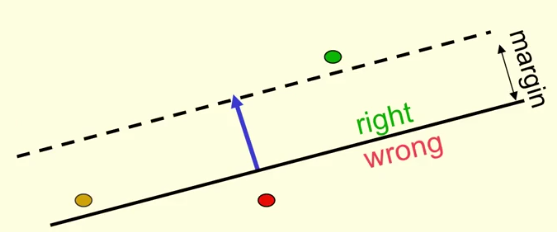
\includegraphics[width=\textwidth]{generously_feasible}
\caption{A generously feasible region.}
\label{fig:generously_feasible}
\end{figure}

Since there is a minimum length of the vectors in the training set, the weight vector much eventually end up being feasible.

\end{document}